\chapter{بنى لويس وأشكال الجزيئات}\label{ch:g10:lewis-and-shape}

\omterm{def:g7:atoms-and-molecules:molecule}{جزيء} ثنائي أكسيد الكربون مستقيم؛ \omterm{def:g7:atoms-and-molecules:molecule}{وجزيء} الماء منحنٍ. وهذا الفرق الوحيد في
الشكل أحد الأسباب التي تجعل الماء، وجزيئاته أخف من \omterm{def:g7:atoms-and-molecules:molecule}{جزيئات} ثنائي أكسيد
الكربون، سائلًا في درجة حرارة الغرفة بينما ثنائي أكسيد الكربون غاز. \omterm{def:g7:atoms-and-molecules:atom}{فالذرات}
في \omterm{def:g7:atoms-and-molecules:molecule}{الجزيء} تمسكها معًا \omterm{def:g9:inside-the-atom:nucleus}{إلكترونات} مشتركة، وطريقة اشتراك \omterm{def:g9:inside-the-atom:nucleus}{الإلكترونات} هي التي
تحدد الشكل. يرسم هذا الفصل \omterm{def:g9:inside-the-atom:nucleus}{الإلكترونات} المشتركة، ومنها يتنبأ بالشكل.

\begin{recall}
\omterm{def:g10:electron-shells:valence}{إلكترونات التكافؤ} هي \omterm{def:g9:inside-the-atom:nucleus}{إلكترونات} \omterm{def:g10:electron-shells:configuration}{الطبقة} الخارجية؛ \omterm{def:g7:atoms-and-molecules:atom}{والذرات} تميل إلى بلوغ \omterm{def:g10:electron-shells:configuration}{التوزيع
الإلكتروني} \omterm{def:g10:electron-shells:family}{لغاز نبيل}، أي ثمانية \omterm{def:g9:inside-the-atom:nucleus}{إلكترونات} في \omterm{def:g10:electron-shells:configuration}{الطبقة} الخارجية (\omterm{def:g10:electron-shells:octet}{قاعدة
الثمانية}) أو اثنين للهيدروجين (\omterm{def:g10:electron-shells:octet}{قاعدة الثنائية})
(\cref{ch:g10:electron-shells}). والنماذج الجزيئية تمثّل \omterm{def:g7:atoms-and-molecules:atom}{الذرات} بكرات
والروابط بعصيّ (\cref{ch:g7:atoms-and-molecules}).
\end{recall}

\section{الرابطة التساهمية}

\begin{definition}[الرابطة التساهمية]\label{def:g10:lewis-and-shape:covalent-bond}
\emph{الرابطة التساهمية}\index{رابطة تساهمية} زوج من \omterm{def:g9:inside-the-atom:nucleus}{الإلكترونات} تتشارك فيه
ذرتان؛ وكل \omterm{def:g7:atoms-and-molecules:atom}{ذرة} تقدّم عادة أحد إلكتروني الزوج. وتحسب الذرتان كلتاهما الزوج
المشترك في طبقتها الخارجية، فتبلغ كل منهما ثنائيتها أو
ثمانيتها.
\end{definition}

\begin{definition}[الأزواج الرابطة والأزواج الحرة]\label{def:g10:lewis-and-shape:lone-pair}
في \omterm{def:g7:atoms-and-molecules:molecule}{الجزيء} تتجمع \omterm{def:g10:electron-shells:valence}{إلكترونات التكافؤ} لكل \omterm{def:g7:atoms-and-molecules:atom}{ذرة} أزواجًا. \emph{الزوج
الرابط}\index{زوج رابط} تتشارك فيه ذرتان ويكوّن \omterm{def:g10:lewis-and-shape:covalent-bond}{رابطة تساهمية}؛ و\emph{الزوج
الحر}\index{زوج حر} يخص \omterm{def:g7:atoms-and-molecules:atom}{ذرة} واحدة ولا يشارك في أي
رابطة.
\end{definition}

\begin{proposition}[كم رابطة تكوّن الذرة]\label{prop:g10:lewis-and-shape:valence}
تكوّن \omterm{def:g7:atoms-and-molecules:atom}{الذرة} من الروابط التساهمية بقدر ما ينقصها من \omterm{def:g9:inside-the-atom:nucleus}{إلكترونات} لإكمال ثنائيتها
أو ثمانيتها:
\begin{center}
\small
\begin{tabular}{lcccc}
\hline
\omterm{def:g7:atoms-and-molecules:atom}{الذرة} & \omterm{def:g10:electron-shells:valence}{إلكترونات التكافؤ} & الروابط & الأزواج الحرة & مثال \\
\hline
H & 1 & 1 & 0 & \ce{H2} \\
C & 4 & 4 & 0 & \ce{CH4} \\
N & 5 & 3 & 1 & \ce{NH3} \\
O & 6 & 2 & 2 & \ce{H2O} \\
Cl & 7 & 1 & 3 & \ce{HCl} \\
\hline
\end{tabular}
\end{center}
\end{proposition}

\section{بنى لويس}

\begin{definition}[بنية لويس]\label{def:g10:lewis-and-shape:lewis-structure}
\emph{بنية لويس}\index{بنية لويس} \omterm{def:g7:atoms-and-molecules:molecule}{لجزيء} تمثّل ذراته برموزها، وكل \omterm{def:g10:lewis-and-shape:lone-pair}{زوج رابط}
بخط بين ذرتين، وكل \omterm{def:g10:lewis-and-shape:lone-pair}{زوج حر} بنقطتين بجانب ذرته.
\end{definition}

\begin{definition}[الروابط الثنائية والثلاثية]\label{def:g10:lewis-and-shape:multiple-bond}
قد تتشارك ذرتان زوجين من \omterm{def:g9:inside-the-atom:nucleus}{الإلكترونات}، أي \emph{رابطة
ثنائية}\index{رابطة ثنائية}، تُرسم بخطين، أو ثلاثة أزواج، أي
\emph{رابطة ثلاثية}\index{رابطة ثلاثية}، تُرسم بثلاثة خطوط.
\end{definition}

\begin{method}[رسم بنية لويس]\label{met:g10:lewis-and-shape:draw}
\begin{enumerate}
  \item اجمع \omterm{def:g10:electron-shells:valence}{إلكترونات التكافؤ} لكل \omterm{def:g7:atoms-and-molecules:atom}{الذرات}، واقسم على اثنين لتحصل على
        عدد الأزواج.
  \item اربط \omterm{def:g7:atoms-and-molecules:atom}{الذرات} بروابط أحادية (الهيدروجين، الذي يكوّن رابطة واحدة،
        يكون دائمًا في الطرف؛ والكربون مركزي في العادة).
  \item ضع الأزواج الباقية أزواجًا حرة، على \omterm{def:g7:atoms-and-molecules:atom}{الذرات} الطرفية أولًا،
        لإكمال ثمانياتها.
  \item إذا بقيت \omterm{def:g7:atoms-and-molecules:atom}{ذرة} دون ثمانية، فحوّل زوجًا حرًا \omterm{def:g7:atoms-and-molecules:atom}{لذرة} مجاورة
        إلى زوج مشترك ثانٍ (أو ثالث).
  \item تحقق: لكل هيدروجين إلكترونان، ولكل \omterm{def:g7:atoms-and-molecules:atom}{ذرة} أخرى 8، وقد استُعملت
        الأزواج كلها.
\end{enumerate}
\end{method}

\begin{example}[ثنائي أكسيد الكربون]\label{ex:g10:lewis-and-shape:co2}
\ce{CO2}: $4 + 2 \times 6 = 16$ \omterm{def:g10:electron-shells:valence}{إلكترون تكافؤ}، أي 8 أزواج. والروابط الأحادية
\ce{O-C-O} تستعمل زوجين؛ و6 أزواج حرة على ذرتي الأكسجين تكملهما، لكن الكربون
لا يبقى له عندئذ إلا 4 \omterm{def:g9:inside-the-atom:nucleus}{إلكترونات}. وتحويل \omterm{def:g10:lewis-and-shape:lone-pair}{زوج حر} من كل أكسجين إلى زوج مشترك
يعطي رابطتين ثنائيتين: فيصير لكل \omterm{def:g7:atoms-and-molecules:atom}{ذرة} ثمانيتها.
\end{example}

\begin{omfigure}
\setchemfig{atom sep=2.0em}
\begin{tabular}{cccccc}
\chemfig{H-H} & \chemfig{H-\charge{0=\:,90=\:,270=\:}{Cl}} & \chemfig{H-\charge{90=\:,270=\:}{O}-H} &
\chemfig{H-\charge{90=\:}{N}(-[6]H)-H} & \chemfig{H-C(-[2]H)(-[6]H)-H} &
\chemfig{\charge{135=\:,225=\:}{O}=C=\charge{45=\:,315=\:}{O}} \\[4pt]
\small \ce{H2} & \small \ce{HCl} & \small \ce{H2O} & \small \ce{NH3} & \small \ce{CH4} & \small \ce{CO2} \\[10pt]
\chemfig{\charge{180=\:}{N}~\charge{0=\:}{N}} & \chemfig{\charge{135=\:,225=\:}{O}=\charge{45=\:,315=\:}{O}} &
\chemfig{C(-[3]H)(-[5]H)=C(-[1]H)-[7]H} & \chemfig{H-C~\charge{0=\:}{N}} &
\chemfig{H-C(-[6]H)=\charge{45=\:,315=\:}{O}} & \\[4pt]
\small \ce{N2} & \small \ce{O2} & \small \ce{C2H4} & \small \ce{HCN} & \small ميثانال \ce{CH2O} &
\end{tabular}

{\small بنى لويس لأحد عشر جزيئًا. كل \omterm{def:g7:atoms-and-molecules:atom}{ذرة} غير الهيدروجين محاطة بأربعة أزواج
(روابط وأزواج حرة): أي بثمانية.}
\end{omfigure}

\section{أشكال الجزيئات}

\begin{proposition}[أزواج الإلكترونات تتباعد قدر الإمكان]\label{prop:g10:lewis-and-shape:shape}
حول \omterm{def:g7:atoms-and-molecules:atom}{الذرة} المركزية تتنافر مجموعات \omterm{def:g9:inside-the-atom:nucleus}{الإلكترونات} --- كل رابطة أحادية أو ثنائية أو
ثلاثية، وكل \omterm{def:g10:lewis-and-shape:lone-pair}{زوج حر} --- وتستقر متباعدة قدر الإمكان. ومن ذلك ينتج شكل
\omterm{def:g7:atoms-and-molecules:molecule}{الجزيء}:
\begin{center}
\small
\begin{tabular}{llll}
\hline
عدد المجموعات حول المركز & منها أزواج حرة & الشكل & مثال \\
\hline
2 & 0 & خطي، الزاوية \ang{180} & \ce{CO2}، \ce{HCN} \\
3 & 0 & مثلثي مستوٍ، الزاوية \ang{120} & \ce{CH2O}، \ce{C2H4} \\
4 & 0 & رباعي الأوجه، الزاوية \ang{109.5} & \ce{CH4} \\
4 & 1 & هرمي & \ce{NH3} \\
4 & 2 & منحنٍ & \ce{H2O} \\
\hline
\end{tabular}
\end{center}
\end{proposition}
\admitted

\begin{remark}[من أين تأتي هذه القاعدة]\label{rem:g10:lewis-and-shape:vsepr}
هذه القاعدة نموذج، وهي تصلح على نحو لافت \omterm{def:g7:atoms-and-molecules:molecule}{للجزيئات} الصغيرة؛ وتُدقَّق، ويُشرح
جزء منها، في كتاب السنة الجامعية الأولى. والأزواج الحرة تشغل حيزًا أكبر قليلًا
من الأزواج الرابطة: فالزاوية في الأمونياك (\ang{106.7}) وفي الماء
(\ang{104.5}) أصغر قليلًا من زاوية الميثان
\ang{109.5}.
\end{remark}

\begin{omfigure}
\begin{tikzpicture}[font=\small]
  % methane, tetrahedral, in perspective
  \begin{scope}
    \node[aC] (c) at (0,0) {};
    \node[aH, minimum size=3.6mm] (hb) at (0.3,-0.12) {};
    \node[aH] (h1) at (0,1.05) {};
    \node[aH] (h2) at (-1.0,-0.45) {};
    \node[aH] (h3) at (0.72,-0.5) {};
    \begin{scope}[on background layer]
      \foreach \h in {h1,h2,h3,hb} \draw[bond] (c.center) -- (\h.center);
    \end{scope}
    \node[aC] at (0,0) {};
    \node at (0,-1.35) {الميثان: رباعي الأوجه};
    \node[font=\footnotesize] at (-0.55,0.55) {\ang{109.5}};
  \end{scope}
  % ammonia, pyramid
  \begin{scope}[xshift=4.2cm]
    \fill[omDef!25] (0,0.2) ellipse (0.18 and 0.45);
    \node[font=\scriptsize, omDef] at (0,1.0) {زوج حر};
    \node[aN] (n) at (0,0) {};
    \node[aH] (h1) at (-0.95,-0.5) {};
    \node[aH] (h2) at (0.7,-0.55) {};
    \node[aH, minimum size=3.6mm] (h3) at (0.25,-0.2) {};
    \begin{scope}[on background layer]
      \foreach \h in {h1,h2,h3} \draw[bond] (n.center) -- (\h.center);
    \end{scope}
    \node[aN] at (0,0) {};
    \node at (0,-1.35) {الأمونياك: هرمي};
  \end{scope}
  % water, bent
  \begin{scope}[xshift=8.4cm]
    \fill[omDef!25, rotate=25] (0,0.2) ellipse (0.16 and 0.42);
    \fill[omDef!25, rotate=-25] (0,0.2) ellipse (0.16 and 0.42);
    \node[aO] (o) at (0,0) {};
    \node[aH] (h1) at (-0.8,-0.58) {};
    \node[aH] (h2) at (0.8,-0.58) {};
    \begin{scope}[on background layer]
      \draw[bond] (o.center) -- (h1.center); \draw[bond] (o.center) -- (h2.center);
    \end{scope}
    \node[aO] at (0,0) {};
    \draw[black!60] (-0.32,-0.23) arc[start angle=216, end angle=324, radius=0.4];
    \node[font=\footnotesize] at (0,-0.65) {\ang{104.5}};
    \node at (0,-1.35) {الماء: منحنٍ};
  \end{scope}
  % carbon dioxide, linear
  \begin{scope}[xshift=12.0cm]
    \node[aO] (a) at (-0.8,0) {}; \node[aC] (c) at (0,0) {}; \node[aO] (b) at (0.8,0) {};
    \begin{scope}[on background layer]
      \foreach \d in {-1.6,1.6} {
        \draw[bond, line width=1.1pt] ([yshift=\d pt]a.center) -- ([yshift=\d pt]c.center);
        \draw[bond, line width=1.1pt] ([yshift=\d pt]c.center) -- ([yshift=\d pt]b.center);}
    \end{scope}
    \node at (0,-1.35) {ثنائي أكسيد الكربون: خطي};
  \end{scope}
\end{tikzpicture}

{\small أشكال أربعة \omterm{def:g7:atoms-and-molecules:molecule}{جزيئات} (الأزواج الحرة ممثَّلة بفصوص مظلَّلة).
% ledger: ang:H2O, ang:NH3
الميثان رباعي الأوجه، والأمونياك هرمي، والماء منحنٍ، وثنائي أكسيد الكربون
مستقيم.}
\end{omfigure}

\begin{omfigure}
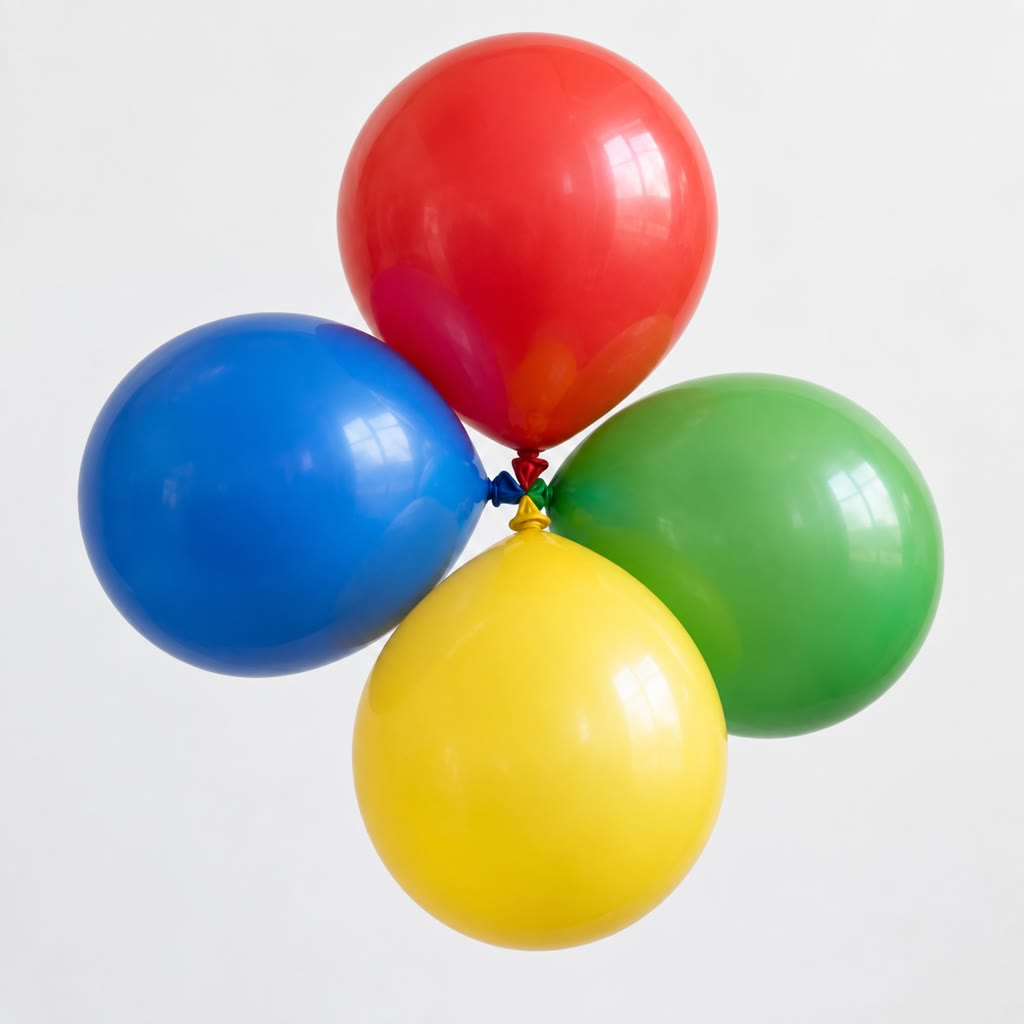
\includegraphics[width=0.38\linewidth]{images/book1/ai/g10-balloons-tetrahedron.jpg}

{\small أربعة بالونات مربوطة معًا يدفع بعضها بعضًا إلى أبعد ما تستطيع؛ فتتجه في
الفضاء إلى رؤوس رباعي أوجه، مثل أزواج \omterm{def:g9:inside-the-atom:nucleus}{الإلكترونات} الأربعة حول \omterm{def:g7:atoms-and-molecules:atom}{ذرة}
الكربون.}
\end{omfigure}

\section{رسم الجزيئات في الفضاء}

\begin{notation}[الأسافين الممتلئة والمتقطعة]\label{not:g10:lewis-and-shape:wedge}
لرسم \omterm{def:g7:atoms-and-molecules:molecule}{جزيء} في الفضاء على ورقة مستوية، تُرسم الرابطة الواقعة في مستوى الورقة
خطًا عاديًا، والرابطة المتجهة نحو القارئ إسفينًا ممتلئًا، والرابطة المتجهة
بعيدًا عنه إسفينًا متقطعًا. فيُرسم الميثان عندئذ كما يلي: رابطتان في المستوى،
وواحدة نحو القارئ وأخرى بعيدًا عنه.
\begin{center}
\chemfig{C(-[2]H)(-[4]H)(<[7]H)(<:[5]H)}
\end{center}
\end{notation}

\section{تمارين}

\begin{exercise}[$\star$]\label{exo:g10:lewis-and-shape:1}
ما \omterm{def:g10:lewis-and-shape:covalent-bond}{الرابطة التساهمية}؟ وما \omterm{def:g10:lewis-and-shape:lone-pair}{الزوج الحر}؟
\end{exercise}

\begin{exercise}[$\star$]\label{exo:g10:lewis-and-shape:2}
كم \omterm{def:g10:lewis-and-shape:covalent-bond}{رابطة تساهمية} يكوّن عادة كل من الهيدروجين والكربون والنيتروجين والأكسجين؟
علّل بقاعدتي الثمانية والثنائية.
\end{exercise}

\begin{exercise}[$\star$]\label{exo:g10:lewis-and-shape:3}
ارسم \omterm{def:g10:lewis-and-shape:lewis-structure}{بنية لويس} لكلوريد الهيدروجين، \ce{HCl}، وعُدّ \omterm{def:g9:inside-the-atom:nucleus}{الإلكترونات} حول
الكلور.
\end{exercise}

\begin{exercise}[$\star$]\label{exo:g10:lewis-and-shape:4}
كم \omterm{def:g10:electron-shells:valence}{إلكترون تكافؤ} يملك \omterm{def:g7:atoms-and-molecules:molecule}{الجزيء} \ce{NH3} في المجموع؟ وكم
زوجًا؟
\end{exercise}

\begin{exercise}[$\star$]\label{exo:g10:lewis-and-shape:5}
أعطِ شكل كل من \ce{CH4} و\ce{NH3} و\ce{H2O} و\ce{CO2}.
\end{exercise}

\begin{exercise}[$\star\star$]\label{exo:g10:lewis-and-shape:6}
ارسم \omterm{def:g10:lewis-and-shape:lewis-structure}{بنية لويس} لكبريتيد الهيدروجين، \ce{H2S} (الكبريت في \omterm{def:g9:periodic-table-first-look:period}{زمرة} الأكسجين)،
وتنبأ بشكله.
\end{exercise}

\begin{exercise}[$\star\star$]\label{exo:g10:lewis-and-shape:7}
ارسم \omterm{def:g10:lewis-and-shape:lewis-structure}{بنية لويس} للنيتروجين، \ce{N2}، متبعًا الطريقة خطوة
خطوة.
\end{exercise}

\begin{exercise}[$\star\star$]\label{exo:g10:lewis-and-shape:8}
ارسم \omterm{def:g10:lewis-and-shape:lewis-structure}{بنية لويس} للميثانول، \ce{CH3OH}، وأعطِ الشكل حول الكربون وحول
الأكسجين.
\end{exercise}

\begin{exercise}[$\star\star$]\label{exo:g10:lewis-and-shape:9}
لماذا يكون \ce{CO2} خطيًا و\ce{H2O} منحنيًا، مع أن في كل منهما \omterm{def:g7:atoms-and-molecules:atom}{ذرة} مركزية
مرتبطة بذرتين أخريين؟
\end{exercise}

\begin{exercise}[$\star\star$]\label{exo:g10:lewis-and-shape:10}
ارسم \omterm{def:g10:lewis-and-shape:lewis-structure}{بنية لويس} للإيثين، \ce{C2H4}، وأعطِ الشكل حول كل \omterm{def:g7:atoms-and-molecules:atom}{ذرة}
كربون.
\end{exercise}

\begin{exercise}[$\star\star$]\label{exo:g10:lewis-and-shape:11}
ارسم \omterm{def:g10:lewis-and-shape:lewis-structure}{بنية لويس} لرباعي كلورو الميثان، \ce{CCl4}، وتنبأ
بشكله.
\end{exercise}

\begin{exercise}[$\star\star\star$]\label{exo:g10:lewis-and-shape:12}
لجزيئين الصيغة \ce{C2H6O}. ارسم \omterm{def:g10:lewis-and-shape:lewis-structure}{بنية لويس} لكل منهما (في أحدهما رابطة O--H،
وفي الآخر سلسلة C--O--C).
\end{exercise}

\begin{exercise}[$\star\star\star$]\label{exo:g10:lewis-and-shape:13}
اشرح، مستعينًا بالأزواج الحرة، لماذا تكون الزاوية في الأمونياك (\ang{106.7})
أصغر منها في الميثان (\ang{109.5})، وفي الماء (\ang{104.5}) أصغر
أيضًا.
\end{exercise}

\begin{exercise}[$\star\star\star$]\label{exo:g10:lewis-and-shape:14}
ارسم \omterm{def:g10:lewis-and-shape:lewis-structure}{بنية لويس} لسيانيد الهيدروجين، \ce{HCN}، وللميثانال،
\ce{CH2O}، وأعطِ شكليهما.
\end{exercise}

\begin{exercise}[$\star\star\star$]\label{exo:g10:lewis-and-shape:15}
الأوزون، \ce{O3}، سلسلة من ثلاث \omterm{def:g7:atoms-and-molecules:atom}{ذرات} أكسجين. عُدّ أزواج التكافؤ فيه، وارسم
\omterm{def:g10:lewis-and-shape:lewis-structure}{بنية لويس} تكون فيها لكل \omterm{def:g7:atoms-and-molecules:atom}{ذرة} أكسجين ثمانيتها (\omterm{def:g10:lewis-and-shape:multiple-bond}{رابطة ثنائية} واحدة، ورابطة أحادية
واحدة). وتنبأ هل \omterm{def:g7:atoms-and-molecules:molecule}{الجزيء} خطي أم
منحنٍ.
\end{exercise}

\section{مسألة: جزيء في مكعب}

\begin{problem}[{مسألة نهاية الأسبوع --- تصميم كرات الكربون في طقم نماذج جزيئية:
بأي زاوية يجب أن تُثقب الثقوب؟}]
\label{pb:g10:lewis-and-shape:1}
% ledger: ang:H2O, ang:NH3
تصنع شركة أطقمًا من النماذج الجزيئية. ويجب أن يكون في كرات الكربون السوداء
أربعة ثقوب، حتى يخرج الميثان والإيثان وسائر \omterm{def:g7:atoms-and-molecules:molecule}{جزيئات} الكربون بالشكل الصحيح.
ويستعمل المهندس حيلة: رباعي الأوجه المنتظم يتسع داخل مكعب، ورؤوسه الأربعة
على أربعة من رؤوس المكعب، وليس اثنان منها على الضلع
نفسه.

\medskip
\noindent\textbf{الجزء الأول --- بنى لويس.}
\begin{enumerate}
  \item ارسم بنى لويس للميثان \ce{CH4}، والأمونياك \ce{NH3}،
        والماء \ce{H2O}.
  \item كم مجموعة من \omterm{def:g9:inside-the-atom:nucleus}{الإلكترونات} تحيط \omterm{def:g7:atoms-and-molecules:atom}{بالذرة} المركزية في كل منها؟
  \item كم منها أزواج حرة؟
  \item لماذا تحتاج كرة الكربون إلى أربعة ثقوب، وكرة الأكسجين (للماء)
        إلى ثقبين فقط؟
  \item نموذج الإيثان، \ce{C2H6}، يستعمل كرتي كربون. ارسم \omterm{def:g10:lewis-and-shape:lewis-structure}{بنية لويس}
        له. كم عصا تربط كرتي الكربون، وكم كرة هيدروجين
        تلزم؟
\end{enumerate}

\medskip
\noindent\textbf{الجزء الثاني --- الأشكال.}
\begin{enumerate}[resume]
  \item أعطِ شكل كل من \omterm{def:g7:atoms-and-molecules:molecule}{الجزيئات} الثلاثة.
  \item الزاويتان المقيستان \ang{106.7} في الأمونياك و\ang{104.5} في
        الماء. اشرح لماذا هما أصغر من زاوية الميثان.
  \item لماذا لا يمكن أن تكون كرة الأكسجين للماء مجرد كرة كربون تُركت فيها
        ثقبان فارغان، إذا أُريد للطقم أن يُظهر الزاوية الحقيقية؟
  \item في ثنائي أكسيد الكربون تكوّن \omterm{def:g7:atoms-and-molecules:atom}{ذرة} الكربون رابطتين ثنائيتين. أي
        زاوية يجب أن تفصل بينهما في النموذج؟
\end{enumerate}

\medskip
\noindent\textbf{الجزء الثالث --- المكعب.}
خذ مكعبًا طول ضلعه $a$. \omterm{def:g7:atoms-and-molecules:atom}{ذرة} الكربون في مركزه؛ \omterm{def:g7:atoms-and-molecules:atom}{وذرات} الهيدروجين الأربع على
أربعة من رؤوس المكعب، وليس اثنتان منها على الضلع نفسه.
\begin{enumerate}[resume]
  \item بيّن أن أي ذرتين من \omterm{def:g7:atoms-and-molecules:atom}{ذرات} الهيدروجين هذه تقعان على طرفي قطر وجه
        من أوجه المكعب. واحسب بمبرهنة فيثاغورس المسافة بينهما بدلالة
        $a$.
  \item طول قطر المكعب كله (من رأس إلى الرأس المقابل) هو
        $a\sqrt{3}$. استنتج المسافة بين \omterm{def:g7:atoms-and-molecules:atom}{ذرة} الكربون \omterm{def:g7:atoms-and-molecules:atom}{وذرة}
        هيدروجين.
  \item خذ $a = \qty{1}{cm}$ في نموذج: أعطِ المسافتين بالسنتيمتر، بمنزلتين
        عشريتين.
  \item لماذا تتساوى المسافات C--H الأربع؟
\end{enumerate}

\medskip
\noindent\textbf{الجزء الرابع --- الزاوية.}
تكوّن \omterm{def:g7:atoms-and-molecules:atom}{ذرة} الكربون C وذرتا الهيدروجين H$_1$ وH$_2$ مثلثًا متساوي
الساقين. لتكن M منتصف H$_1$H$_2$.
\begin{enumerate}[resume]
  \item اشرح لماذا يكون المثلث C\,M\,H$_1$ قائمًا في M.
  \item احسب، في هذا المثلث القائم، جيب الزاوية
        $\widehat{\text{M\,C\,H}_1}$، وهي نصف الزاوية H--C--H.
  \item استنتج نصف الزاوية، ثم الزاوية H--C--H، بمنزلة عشرية
        واحدة.
  \item قارن بزاوية الجدول في هذا الفصل.
  \item اذكر الزاوية التي يجب أن تُثقب بها ثقوب كرة
        الكربون.
\end{enumerate}
\end{problem}
